\documentclass{article}

\usepackage{timing-diagrams}

\usepackage{pifont}

\begin{document}

\section{Basic diagram}

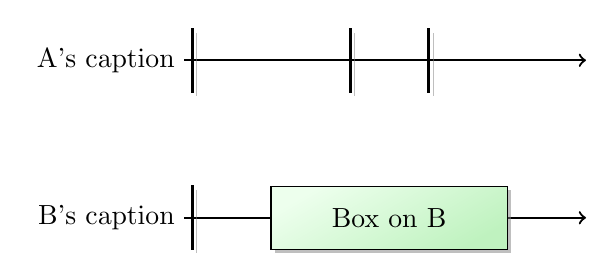
\begin{tikzpicture}
  % Define timelines with their names, and ordinate as #2:
  \tline{A}{2};
  \tline{B}{0};
  % Actually draw the timelines (#2 is the horizontal length):
  \ttimeline{A}{5};
  \ttimeline{B}{5};
  % Provide captions for timelines:
  \tcaption{A}{A's caption};
  \tcaption{B}{B's caption};
  
  % Draw the actual content:
  % tick = vertical line accros the timeline
  \ttick{A};
  % advance time
  \tskip{A}{2};
  % This one will be drawn 2 time units after the previous, because of
  % the \tskip:
  \ttick{A};
  
  % One more with the same principle:
  \tskip{A}{1};
  \ttick{A};

  % Same as above, but on timeline B:
  \ttick{B};
  \tskip{B}{1};
  % \tbox creates a box with non-null width, and text inside:
  \tbox{B}{3}{Box on B};
\end{tikzpicture}

\section{Timeline, ticks and tasks}

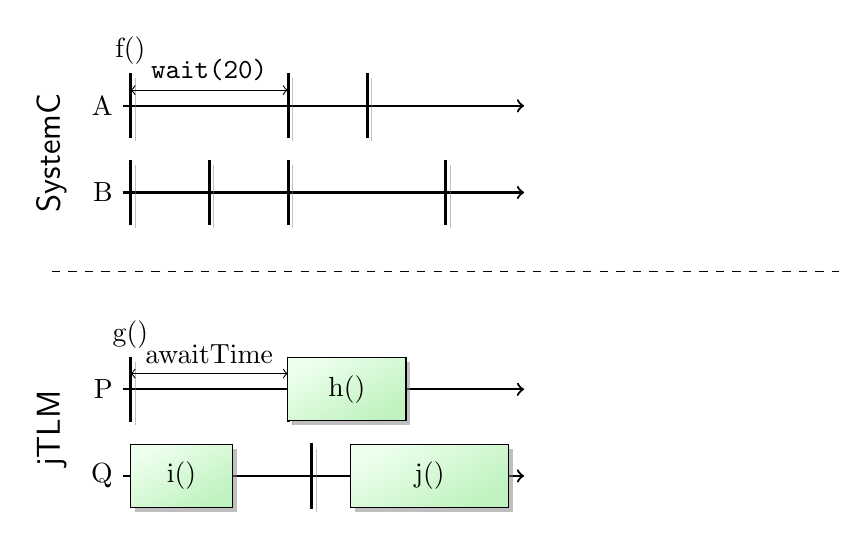
\begin{tikzpicture}
  \draw (-1,1.5)  node[rotate=90] (systemc) {\textsf{\large SystemC}};
  \draw[dashed] (-1,0) -- (9,0);
  \draw (-1,-2) node[rotate=90] (jtlm) {\textsf{\large jTLM}};

  % SystemC
  \tline{A}{2.1};
  \tcaption{A}{A};
  \tline{B}{1};
  \tcaption{B}{B};

  \ttimeline{A}{5};
  \ttimeline{B}{5};

  % jTLM
  \tline{P}{-1.5};
  \tcaption{P}{P};
  \tline{Q}{-2.6};
  \tcaption{Q}{Q};

  \ttimeline{P}{5};
  \ttimeline{Q}{5};


  \ttick{A};
  \ttextU{A}{f()};
  \tskiptext{A}{2}{\texttt{wait(20)}};
  \ttick{A};
  \tskip{A}{1};
  \ttick{A};

  \ttick{B}
  \tskip{B}{1};
  \ttick{B};
  \tskip{B}{1};
  \ttick{B};
  \tskip{B}{2};
  \ttick{B};

  \ttick{P}
  \ttextU{P}{g()};
  \tskiptext{P}{2}{awaitTime}
  \ttick{P};

  \tbox{P}{1.5}{h()};

  % just so that the final picture looks pretty
  \tbox{Q}{1.3}{i()};
  \tskip{Q}{1};
  \ttick{Q};
  \tskip{Q}{.5};
  \tbox{Q}{2}{j()};

\end{tikzpicture}

\section{Annotations over a diagram}

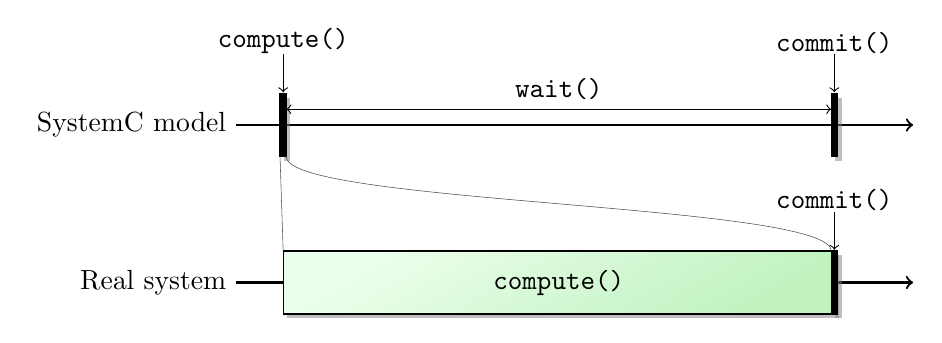
\begin{tikzpicture}
  \tline{real}{0};
  \tline{model}{2};

  \ttimeline{real}{8.5};
  \ttimeline{model}{8.5};

  \tcaption{real}{Real system};
  \tcaption{model}{SystemC model};

  \tskip{real}{.5};
  \tskip{model}{.5};

  \path (currentrealU) coordinate (endzooma);
  \tbox{real}{7}{\texttt{compute()}};
  \path (currentrealU) ++(-.04, 0) coordinate (endzoomb);
  \tstrongtick{real};
  \ttextarrowU{real}{\texttt{commit()}};

  \tstrongtick{model};
  \path (currentmodelL) ++(-.04, 0) coordinate(startzooma);
  \path (currentmodelL) ++( .04, 0) coordinate(startzoomb);
  \ttextarrowU{model}{\texttt{compute()}};
  \tskip{model}{.04};
  \tskiptext{model}{6.92}{\texttt{wait()}};
  \tskip{model}{.04};
  \tstrongtick{model};
  \ttextarrowU{model}{\texttt{commit()}};

  \path (startzoomb -| endzoomb) coordinate (topright);
  \path (barycentric cs:startzoomb=.5,endzooma=.5) coordinate (tmpa);
  \path (barycentric cs:topright=.5,endzoomb=.5) coordinate (tmpb);
  \draw[very thin,color=black!70!white] (startzooma) -- (endzooma);
  \draw[very thin,color=black!70!white] (startzoomb) .. controls (tmpa) and (tmpb) .. (endzoomb);
\end{tikzpicture}

\section{Annotations with callouts, synchronizations between timelines}

\newcommand{\one}{\raisebox{-2pt}{\large\ding{192}}}
\newcommand{\two}{\raisebox{-1.5pt}{\large\ding{193}}}
\newcommand{\three}{\raisebox{-2pt}{\large\ding{194}}}
\tikzstyle{arrow}=[->,line width=.05cm,draw=red!90!blue!60!black]

\begin{tikzpicture}[scale=.8]
  \tline{A}{3};
  \tcaption{A}{A};
  \tline{B}{2};
  \tcaption{B}{B};
  \tline{C}{1};
  \tcaption{C}{C};
  \tline{T}{-1.5}
  \tcaption{T}{OS thread};

  \ttimeline{A}{10};
  \ttimeline{B}{10};
  \ttimeline{C}{10};
  \ttimeline{T}{10};

  \tbox{B}{1}{};
  \tcatchup{C}{B};
  %
  \tbox{C}{1}{};
  \tcalloutU[(-.8,2.5)]{C}{\texttt{during(42, routine);}}
  %
  %
  \tcatchup{B}{C};
  \tcatchup{T}{C};
  \draw[arrow] (currentCL) -- node[left] {
    \begin{tabular}{r}
      \one{} create\\thread
    \end{tabular}
  } (currentTU);
  \tbox{T}{4}{\texttt{routine}};
  %
  %
  \tskiptextL{C}{4}{\two{} \texttt{wait(42)}\vspace{-2em}};
  %
  %
  \tbox{B}{1.5}{};
  \tcatchup{A}{B};
  \tbox{A}{1}{};
  \tcatchup{B}{A};
  \tbox{B}{1}{};
  %
  %
  \draw[arrow] (currentTU) -- node[right] {
    \begin{tabular}{l}
      \three{} join\\thread
    \end{tabular}
  } (currentCL);
  \tbox{C}{1}{};
  %
  %
  \tcatchup{A}{C};
  \tbox{A}{1}{};
  \tcatchup{B}{A};
  \tbox{B}{1}{};
  %
\end{tikzpicture}

\section{Arrows between timelines}


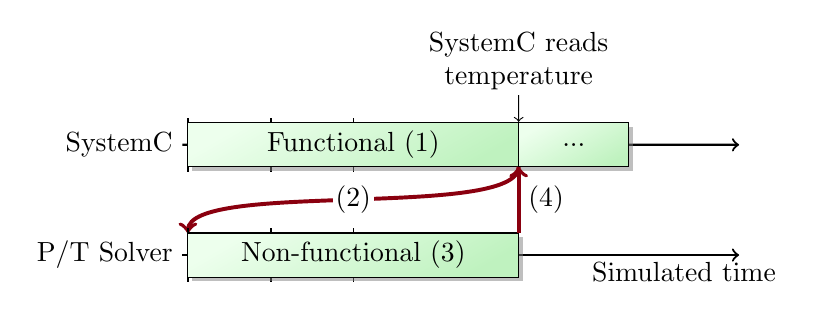
\begin{tikzpicture}[scale=.7]
  \tline{sc}{2};
  \tcaption{sc}{SystemC};

  \tline{ace}{0};
  \draw (currentace) ++ (9,-.3) node {Simulated time};

  \tcaption{ace}{P/T Solver};

  \ttimeline{sc}{10};
  \ttimeline{ace}{10};

  \tremember{sc}{before};
  \tlonglighttick{sc};
  \tskip{sc}{1.5};
  \tlonglighttick{sc};
  \tskip{sc}{1.5};
  \tlonglighttick{sc};
  \tskip{sc}{2};
  \trecall{sc}{before};
  \tbox{sc}{6}{Functional (1)};

  \ttextarrowU{sc}{\begin{tabular}{c}
      SystemC reads\\temperature
    \end{tabular}
  };

  \tarrowUL{sc}{ace}{};
  \draw (tmpmid) node[fill=white,inner sep=1pt] {(2)};
  \tremember{ace}{before};
  \tlonglighttick{ace};
  \tskip{ace}{1.5};
  \tlonglighttick{ace};
  \tskip{ace}{1.5};
  \tlonglighttick{ace};
  \tskip{ace}{2};
  \trecall{ace}{before};
  \tbox{ace}{6}{Non-functional (3)};

  \tarrowLU{ace}{sc}{};
  \draw (tmpmid) node[anchor=west] {(4)};

  \tbox{sc}{2}{...};
\end{tikzpicture}

\vspace{1em}

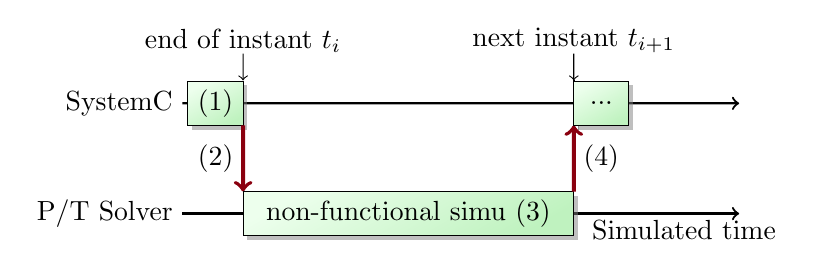
\begin{tikzpicture}[scale=.7]
  \tline{sc}{2};
  \tcaption{sc}{SystemC};

  \tline{ace}{0};
  \tcaption{ace}{P/T Solver};

  \draw (currentace) ++ (9,-.3) node {Simulated time};

  \ttimeline{sc}{10};
  \ttimeline{ace}{10};

  \tbox{sc}{1}{(1)};
  \ttextarrowU{sc}{end of instant $t_{i}$};
  \tcatchup{ace}{sc};
  \coordinate (sceoi) at (currentscL);

  \tskip{sc}{6};
  \ttick{sc};
  \ttextarrowU{sc}{next instant $t_{i+1}$};

  \tarrowCoord{(sceoi)}{(currentaceU)}{};
  \draw (tmpmid) node[anchor=east] {(2)};
  \tbox{ace}{6}{non-functional simu (3)};
  % \tcalloutL{ace}{No IT};
  \ttick{sc};
  \tarrowLU{ace}{sc}{};
  \draw (tmpmid) node[anchor=west] {(4)};
  % \tcalloutU{sc}{Continue};
  \tbox{sc}{1}{...};

\end{tikzpicture}

\section{Events as vertical arrows, mix between timing diagrams and others}

\begin{tikzpicture}
  \tline{S}{6};
  \tline{M}{5};
  \tline{E}{2};
  \tline{T}{0}
  \tline{F}{-2};
  \tline{Eb}{-5};
  \tline{Tb}{-7}

  \coordinate (n1) at (-2.5,-.5);
  \coordinate (n2) at (-2.5,4);
  \draw [decoration={brace,amplitude=10pt},decorate] (n1) to (n2);

  \coordinate (o1) at (-2.5,-7.5);
  \coordinate (o2) at (-2.5,-1.5);
  \draw [decoration={brace,amplitude=10pt},decorate] (o1) to (o2);

  \draw (barycentric cs:n1=.5,n2=.5) ++(-10pt,0) node[anchor=south,rotate=90] {\large\textsf{(a) Naive Temperature Model}};
  \draw (barycentric cs:o1=.5,o2=.5) ++(-10pt,0) node[anchor=south,rotate=90] {\large\textsf{(b) Proposed Approach}};

  \tcaption{S}{Real System};
  \ttimeline{S}{8};

  \tskip{S}{.3};

  \tstartbrace{S};
  \tevent{S}; \tskip{S}{1.5};
  \tevent{S}; \tskip{S}{1.3};
  \tevent{S}; \tskip{S}{1.2};

  \tendbrace{S}{\texttt{f(); wait(40);}};
  \tstartbrace{S};

  \tskip{S}{.2};
  \tevent{S}; \tskip{S}{.8};
  \tevent{S}; \tskip{S}{.7};
  \tevent{S}; \tskip{S}{.5};
  \tevent{S}; \tskip{S}{.5};
  \tevent{S}; \tskip{S}{.8};
  \tevent{S};

  \tendbrace{S}{\texttt{g(); wait(35);}};



  \tcaption{M}{
    \begin{tabular}{r}
      Loosely-Timed\\Model
    \end{tabular}
  };
  \ttimeline{M}{8};
  \tskip{M}{.3};
  \foreach \x in {10,0,-10} {
    \teventA{M}{\x};
  }
  \tskip{M}{4};
  \foreach \x in {25,15,5,-5,-15,-25} {
    \teventA{M}{\x};
  }
  \tskip{M}{2.5};


  \tcaption{E}{Energy};
  \ttimeline{E}{8};

  \draw[red!50!black,thick] (currentE) ++(0,.3) -- ++(.3,0) --
  node[right] {+3} ++(0,.6) -- ++(4,0) --
  node[right] {+6} ++(0,1.2) -- node[near end,below]{total=9} ++(3.5,0)
  ;


  \tcaption{T}{Temperature};

  \ttimeline{T}{8};
  \draw[blue!50!black,thick] (currentT) ++(0,.3) -- ++(.3,0) --
  coordinate[at end](peak1) ++(0,.6) .. controls +(1,-.2) .. ++(4,-.3) --
  coordinate[at end](peak2) ++(0,1) .. controls +(1,-.5) .. ++(3.5,-.8)
  ;



  \draw (peak1) node[draw,circle,thick](peak1){};
  \draw (peak2) node[draw,circle,thick](peak2){};
  \draw (barycentric cs:peak1=.5,peak2=.5) ++(0,.1) node[inner sep=0](peaks){
    \begin{tabular}{c}
      Unrealistic\\peaks
    \end{tabular}
  };
  \draw [arrow] (peaks) -- (peak1);
  \draw [arrow] (peaks) -- (peak2);


  \tcaption{F}{Frequency};
  \ttimeline{F}{8};
  \tskip{F}{.3};
  \tbox{F}{4}{$\frac{3}{40}$ trans/sec};
  \tbox{F}{3.5}{$\frac{6}{35}$ trans/sec};


  \tcaption{Eb}{Energy};
  \ttimeline{Eb}{8};

  \draw[red!50!black,thick] (currentEb) ++(0,.3) -- ++(.3,0) --
  ++(4,.6)
  -- node[at end,right]{total=9} ++(3.5,1.2)
  ;


  \tcaption{Tb}{Temperature};

  \ttimeline{Tb}{8};
  \draw[blue!50!black,thick] (currentTb) ++(0,.3) -- coordinate[at end](start)++(.3,0);
  \path (start)
  ++(4,.6) coordinate (x1)
  ++(3.5,.3) coordinate(x2);
  \draw[blue!50!black,thick,bend left=5] (start) to (x1);
  \draw[blue!50!black,thick,bend left=5] (x1) to (x2);
  ;

\end{tikzpicture}

\end{document}

%%% Local Variables:
%%% mode: latex
%%% TeX-master: t
%%% End:
